% ===================== 4. EXACT — CP-SAT =====================
\section{Lời giải chuẩn xác (Exact Method) với OR-Tools CP-SAT}
\label{sec:exact}

Tầng Exact cung cấp nghiệm tối ưu \emph{có chứng nhận} ở quy mô nhỏ --- vừa là lời
giải cho dữ liệu khoa/viện, vừa là \emph{thước đo vàng} để chấm điểm các tầng xấp
xỉ (Mục~\ref{sec:results}).

\subsection{Mô hình toán học: từ quy hoạch nguyên sang quy hoạch ràng buộc}
Công thức~\eqref{eq:c1}--\eqref{eq:obj} là một mô hình quy hoạch nguyên (ILP). Tuy
nhiên, biểu diễn trực tiếp các họ ràng buộc xung đột~\eqref{eq:c3}--\eqref{eq:c4} sinh
ra hàng vạn bất đẳng thức (một cho mỗi cặp phòng/giáo viên $\times$ tiết) và một mô
hình lỏng lẻo. Ta chuyển sang \emph{quy hoạch ràng buộc} (CP), nơi cấu trúc thời
gian được biểu diễn cô đọng và có bộ truyền lan ràng buộc (propagator) chuyên dụng.

\subsection{Hiện thực hóa bằng Interval Variables và AddNoOverlap}
Với mỗi cặp (lớp $i$, phòng $r$) khả thi ($c_r\ge s_i$):
\begin{itemize}
  \item biến hiện diện $b_{i,r}\in\{0,1\}$;
  \item biến bắt đầu $\text{start}_{i,r}$ ràng buộc chỉ nhận giá trị trong
  $\mathcal{S}(t_i)$ (qua \texttt{AddAllowedAssignments}) --- nơi cài đặt ràng buộc
  logic;
  \item \emph{Optional Interval} $\text{intv}_{i,r}$ --- khối thời lượng $t_i$ chỉ
  ``tồn tại'' khi $b_{i,r}=1$.
\end{itemize}
Khi đó hai họ ràng buộc xung đột thu gọn thành các lời gọi \emph{không-chồng-lấn}:
\begin{align}
  \opt{AddNoOverlap}\big(\{\text{intv}_{i,r} : i\}\big) &\quad \forall r
  &&\text{(mỗi phòng)},\\
  \opt{AddNoOverlap}\big(\{\text{intv}_{i,r} : g_i=g\}\big) &\quad \forall g
  &&\text{(mỗi giáo viên)},
\end{align}
với $\sum_r b_{i,r}=a_i$ và mục tiêu \texttt{Maximize}$(\sum_i a_i)$. Cách này giảm
mạnh số ràng buộc tường minh và để propagator của CP-SAT xử lý xung đột thời gian
hiệu quả hơn nhiều so với ILP tương đương.

\subsection{Tăng tốc bằng Warm-start từ nghiệm Greedy}
Trước khi giải, ta nạp nghiệm Greedy làm \emph{gợi ý} (\texttt{AddHint}, không phải
ràng buộc cứng): $a_i\!\leftarrow\!1$, $b_{i,r}\!\leftarrow\!\mathbf{1}[r{=}r^{g}_i]$,
$\text{start}\!\leftarrow\!u^{g}_i$. Solver có ngay một cận dưới khả thi để cắt
nhánh mạnh hơn, không phí thời gian dò nghiệm khả thi đầu tiên, và đảm bảo kết quả
không bao giờ tệ hơn Greedy.

\subsection{Giới hạn co giãn: bức tường tổ hợp}
\label{sec:cpsat-limit}
Số biến tăng tuyến tính $\mathcal{O}(N\cdot M\cdot\max_i|\mathcal{S}(t_i)|)$, còn
chi phí \emph{chứng minh} tối ưu tăng theo hàm mũ. Trên dữ liệu \emph{thưa}, nhờ
warm-start CP-SAT vẫn giải tối ưu tới $N=600$ (Hình~\ref{fig:cpsat}); bức tường chỉ
lộ ra trên dữ liệu \emph{nghẽn} (Bảng~\ref{tab:cpsat-real}).

\begin{figure}[H]
  \centering
  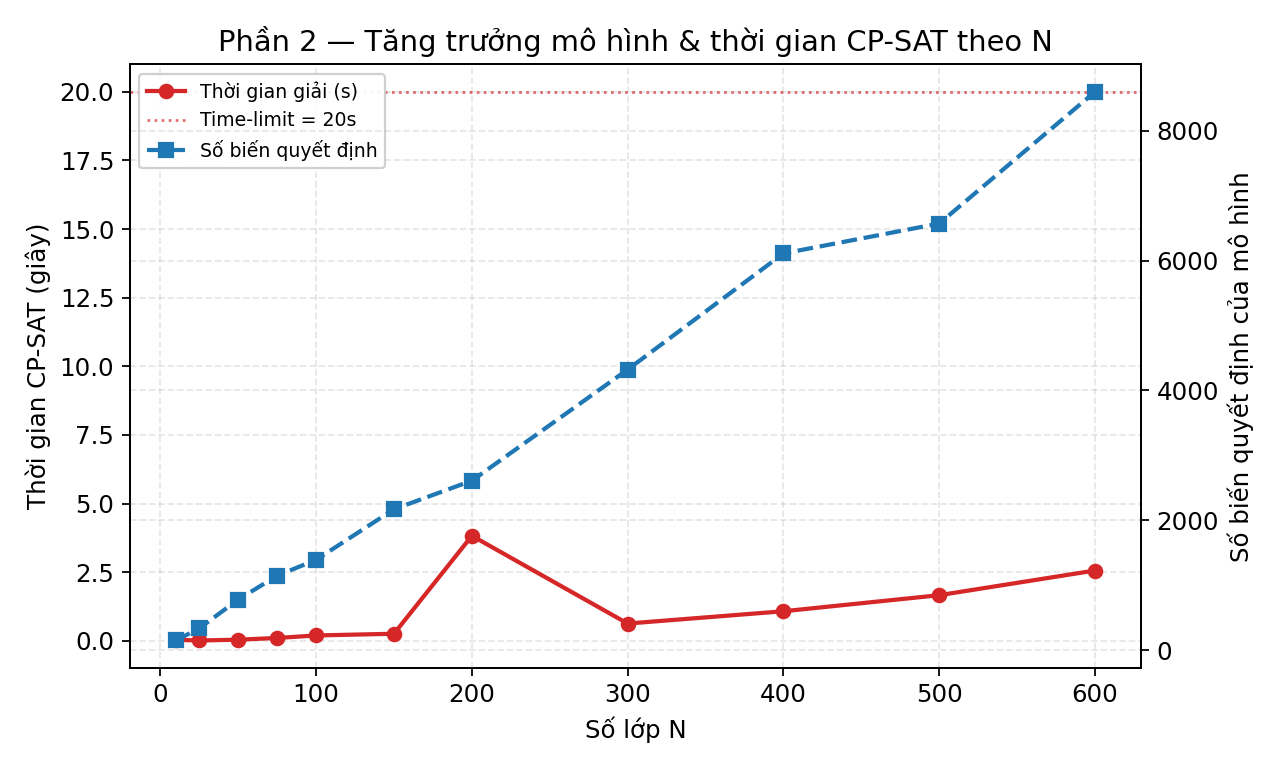
\includegraphics[width=0.74\textwidth]{figures/cpsat_scaling.png}
  \caption{Dữ liệu thưa: số biến (xanh) tăng tuyến tính theo $N$, nhưng thời gian
  giải (đỏ) vẫn xa dưới time-limit. Kích thước một mình không đánh gục CP-SAT.}
  \label{fig:cpsat}
\end{figure}

\begin{table}[ht]
\centering\small
\caption{CP-SAT trên dữ liệu ngẫu nhiên ``loose'' ($M=8$): số biến và thời gian
tăng theo $N$, vẫn chứng minh được tối ưu.}
\label{tab:cpsat-scaling}
\begin{tabular}{rrrlrr}
\toprule
$N$ & Số biến & Thời gian (s) & Trạng thái & $Q$ (obj) & Gap \\
\midrule
10 & 152 & 0.04 & OPTIMAL & 10 & 0 \\
25 & 339 & 0.01 & OPTIMAL & 25 & 0 \\
50 & 782 & 0.04 & OPTIMAL & 48 & 0 \\
75 & 1149 & 0.10 & OPTIMAL & 69 & 0 \\
100 & 1394 & 0.20 & OPTIMAL & 98 & 0 \\
150 & 2172 & 0.26 & OPTIMAL & 146 & 0 \\
200 & 2612 & 3.83 & OPTIMAL & 198 & 0 \\
300 & 4322 & 0.63 & OPTIMAL & 232 & 0 \\
400 & 6110 & 1.08 & OPTIMAL & 255 & 0 \\
500 & 6570 & 1.66 & OPTIMAL & 294 & 0 \\
600 & 8598 & 2.56 & OPTIMAL & 306 & 0 \\
\bottomrule
\end{tabular}
\end{table}

\begin{table}[ht]
\centering\small
\caption{CP-SAT trên dữ liệu thực nghẽn tài nguyên (time-limit $20$s). Khi $N$
lớn, solver chỉ đạt \textsc{feasible} với gap dương: không kịp chứng minh tối ưu.}
\label{tab:cpsat-real}
\begin{tabular}{lrrrrlrrrr}
\toprule
Instance & $N$ & $M$ & Số biến & Wall (s) & Trạng thái & Greedy & $Q$ & Cận trên & Gap \\
\midrule
\texttt{hustack01} & 200 & 10 & 3074 & 20.36 & FEASIBLE & 182 & 196 & 197 & 1 \\
\texttt{hustack02} & 500 & 50 & 38868 & 20.51 & FEASIBLE & 410 & 410 & 418 & 8 \\
\texttt{test08} & 1000 & 50 & 60002 & 20.93 & FEASIBLE & 959 & 961 & 1000 & 39 \\
\bottomrule
\end{tabular}
\end{table}


\noindent Kết quả Bảng~\ref{tab:cpsat-real} là minh chứng cho luận điểm trung tâm:
đối lập với dữ liệu thưa (tối ưu tới $N{=}600$), trên cả ba instance thực nghẽn tài
nguyên CP-SAT \emph{không đóng được khoảng cách} trong $20$s --- đều dừng ở
\textsc{feasible} với gap dương ngay cả khi đã warm-start (\texttt{hustack01}
$N{=}200$ gap $1$; \texttt{hustack02} $N{=}500$ gap $8$; \texttt{test08} $N{=}1000$
gap $39$). Đây là cơ sở định lượng cho ngưỡng $N\le 100$ của bộ định tuyến: vượt
ngưỡng, nguy cơ chỉ nhận nghiệm \textsc{feasible} là quá cao, buộc chuyển sang Local
Search (Mục~\ref{sec:ls}) và ALNS (Mục~\ref{sec:alns}).
